\setcounter{ExampleCounter}{1}
In reality, straight lines are rare; this is as true with data as it is with stone formations.  Real data hardly ever follows such a simple rule, but whenever we can, we like to use lines to approximate real trends because straight lines are easy to work with.

\begin{center}
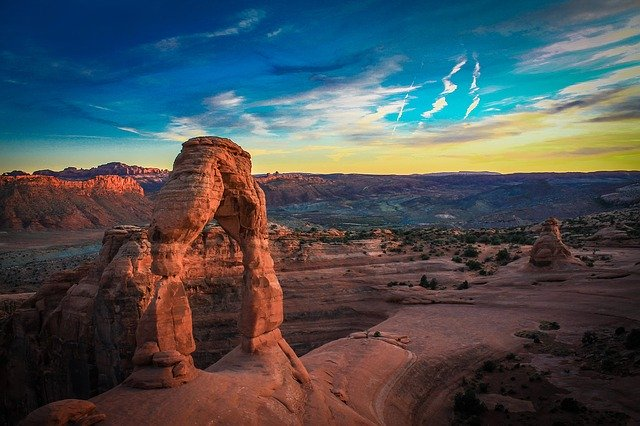
\includegraphics[width=0.8\textwidth]{StoneArch}
\end{center}

However, as we found at the end of the previous section, linear models will not work in every situation, and trying to force a linear trend on real data often leads to nonsensical results.  For the rest of this chapter, we'll study other models--using slightly more complicated formulas--that can be used when the data does not follow a linear trend.

Picking which model to use is a hard question, and this decision is usually based on looking at a graph and looking for a pattern, or trying multiple models and seeing which gives the best results.  That kind of decision is largely beyond the scope of this chapter; we'll focus on learning some basic features of a few different models, and the questions in each section will specify which kind of model to use.

We'll discuss three types of non-linear models:
\begin{enumerate}
\item Quadratic Models
\item Exponential Models
\item Logistic Models
\end{enumerate}

This section will focus on quadratic models, and the last two types will be the topics of the remaining sections in this chapter.

\subsection{Quadratic Models: Parabolas}
\marginnote{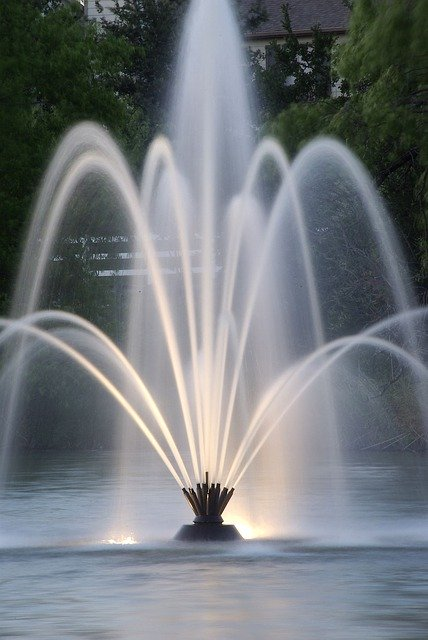
\includegraphics[width=1.5in]{WaterParabola}}
The next time you use a water fountain, watch the path that the water follows.  There's a certain elegance to this arch, and we have a special name for it: a \textbf{parabola}.  Every time a baseball player throws a ball, that ball's path follows this same pattern.  In fact, every time anything is launched or thrown, it follows a parabolic arch.

It turns out that this shape comes from a simple mathematical operation: \emph{squaring}.  Yes, that's it; when you square numbers, this pattern emerges.

Of course, that's not clear immediately, so let's do a simple experiment: square the whole numbers from 0 to 4, as well as the matching negative numbers.  We can arrange our results in a table like this:
\begin{center}
\begin{tabular}{c | c c c c c c c c c}
$x$ & $-4$ & $-3$ & $-2$ & $-1$ & 0 & 1 & 2 & 3 & 4\\
& & & & & & & & & \\
\hline
& & & & & & & & & \\
$x^2$ & 16 & 9 & 4 & 1 & 0 & 1 & 4 & 9 & 16
\end{tabular}
\end{center}

Notice the symmetry in the results: when we square 2 and $-2$, for instance, we get the same result, because multiplying two negative numbers results in a positive answer.  Look at the picture of the fountain in the margin; one of the main features of a parabola is its symmetry, and we're already starting to see that emerge.
\pagebreak

Just like we did in the previous section, let's graph these results and see what visual pattern we can observe.
\begin{center}
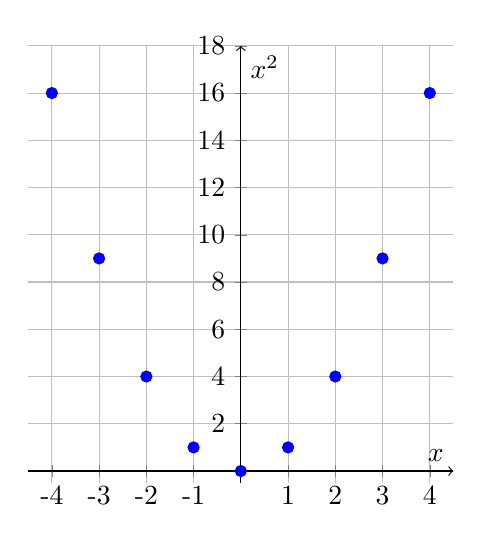
\begin{tikzpicture}
\begin{axis}[
    xmin=-4.5, xmax=4.5,
    ymin=-0.5, ymax=18,
    axis lines=center,
    axis on top=false,
    domain=0:1,
    x=0.6cm,
    y=0.3cm,
    xtick={-4,-3,...,4},
    xticklabels={-4,-3,...,4},
    ytick={0,2,...,18},
    yticklabels={0,2,...,18},
    axis lines=middle,
    axis line style={->},
    %x label style={at={(axis description cs:0.5,-0.1)},anchor=north},
    %y label style={at={(axis description cs:-0.1,.5)},rotate=90,anchor=south},
    xlabel={$x$},
    ylabel={$x^2$},
    grid=major
    ]
	\addplot [blue,only marks,mark size=2] table {
	-4 16
	-3 9
	-2 4
	-1 1
	0 0
	1 1
	2 4
	3 9
	4 16
	};
\end{axis}
\end{tikzpicture}
\end{center}

And if we connect the dots by filling in the results we would get if we applied this same rule to non-whole numbers, what do we get?

\begin{center}
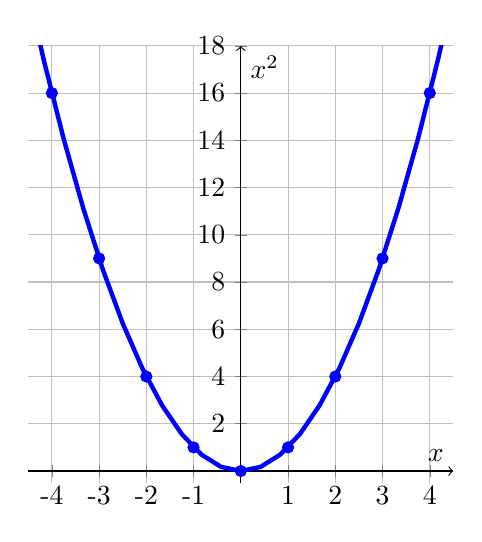
\begin{tikzpicture}
\begin{axis}[
    xmin=-4.5, xmax=4.5,
    ymin=-0.5, ymax=18,
    axis lines=center,
    axis on top=false,
    domain=0:1,
    x=0.6cm,
    y=0.3cm,
    xtick={-4,-3,...,4},
    xticklabels={-4,-3,...,4},
    ytick={0,2,...,18},
    yticklabels={0,2,...,18},
    axis lines=middle,
    axis line style={->},
    %x label style={at={(axis description cs:0.5,-0.1)},anchor=north},
    %y label style={at={(axis description cs:-0.1,.5)},rotate=90,anchor=south},
    xlabel={$x$},
    ylabel={$x^2$},
    grid=major
    ]
	\addplot [blue,only marks,mark size=2] table {
	-4 16
	-3 9
	-2 4
	-1 1
	0 0
	1 1
	2 4
	3 9
	4 16
	};
	\addplot [blue, ultra thick, domain=-5:5] {x^2};
\end{axis}
\end{tikzpicture}
\end{center}

Look at that: we got exactly the same shape as the water rising and falling in the fountain (although flipped upside-down).  It's amazing what beauty can come from such a simple mathematical rule: when you start squaring numbers, you find a parabolic curve, and it turns out that this curve governs much of the motion we see around us every day.

Now, by comparing this graph with the picture of the fountain, we can observe that while parabolas all have the same structure, there are differences in the exact paths.  For instance, some of the jets in the fountain are aimed higher than others, leading to taller, narrower arches, while the lower jets create shorter, wider arches.  And the graph shows a parabola that is oriented in the opposite direction.

Where do these differences come from?  It's important to remember that the basic structure of the parabola is generated by squaring the inputs (we used $t$ in the previous section; these are the values for which we want to make predictions) to get $x^2$ (or $t^2$).  A more general version of this function (and the formula we'll use when we start building quadratic models) is
\[f(x) = ax^2 + bx + c\]
or, in a form that is more similar to what we used in the last section,
\[P_t = at^2 + bt + c.\]

Notice that if we set $a=1$, $b=0$, and $c=0$, this simplifies to $f(x) = x^2$, which is the one we graphed above (the notation $f(x)=$ simply means that we're thinking of this as a function, a rule that takes inputs $x$ and yields outputs, as we did in the table above).
\vfill
\pagebreak

When we start changing the values of $a$, $b$, and $c$, that's when the variations among different parabolic shapes start to appear.  Here are a few examples:
\begin{center}
\begin{tabular}{c | c}
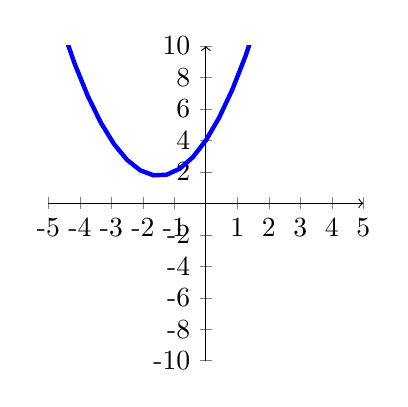
\begin{tikzpicture}
\begin{axis}[
    xmin=-5, xmax=5,
    ymin=-10, ymax=10,
    axis lines=center,
    axis on top=false,
    domain=0:1,
    x=0.4cm,
    y=0.2cm,
    xtick={-5,-4,...,5},
    xticklabels={-5,-4,...,5},
    ytick={-10,-8,...,10},
    yticklabels={-10,-8,...,10},
    axis lines=middle,
    axis line style={->},
    %x label style={at={(axis description cs:0.5,-0.1)},anchor=north},
    %y label style={at={(axis description cs:-0.1,.5)},rotate=90,anchor=south},
    %xlabel={$x$},
    %ylabel={$x^2$},
    %grid=major
    ]
	\addplot [blue,ultra thick,domain=-5:5] {x^2 + 3*x + 4};
\end{axis}
\end{tikzpicture}
\hspace*{0.5in}
& 
\hspace*{0.5in}
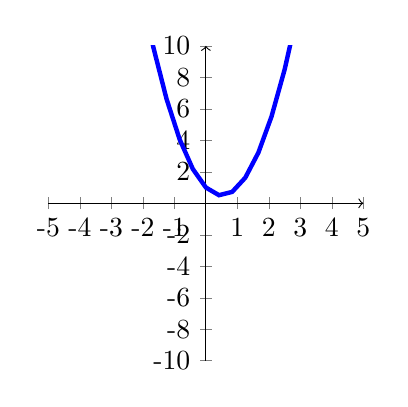
\begin{tikzpicture}
\begin{axis}[
    xmin=-5, xmax=5,
    ymin=-10, ymax=10,
    axis lines=center,
    axis on top=false,
    domain=0:1,
    x=0.4cm,
    y=0.2cm,
    xtick={-5,-4,...,5},
    xticklabels={-5,-4,...,5},
    ytick={-10,-8,...,10},
    yticklabels={-10,-8,...,10},
    axis lines=middle,
    axis line style={->},
    %x label style={at={(axis description cs:0.5,-0.1)},anchor=north},
    %y label style={at={(axis description cs:-0.1,.5)},rotate=90,anchor=south},
    %xlabel={$x$},
    %ylabel={$x^2$},
    %grid=major
    ]
	\addplot [blue,ultra thick,domain=-5:5] {2*x^2 - 2*x +1};
\end{axis}
\end{tikzpicture}\\
$a=1$, $b=3$, $c=4$ \hspace*{0.5in} & \hspace*{0.5in} $a=2$, $b=-2$, $c=1$\\
$x^2 + 3x + 4$ \hspace*{0.5in} & \hspace*{0.5in} $2x^2 - 2x + 1$\\
& \\
\hline
& \\
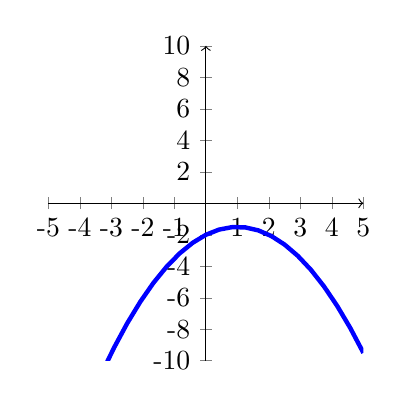
\begin{tikzpicture}
\begin{axis}[
    xmin=-5, xmax=5,
    ymin=-10, ymax=10,
    axis lines=center,
    axis on top=false,
    domain=0:1,
    x=0.4cm,
    y=0.2cm,
    xtick={-5,-4,...,5},
    xticklabels={-5,-4,...,5},
    ytick={-10,-8,...,10},
    yticklabels={-10,-8,...,10},
    axis lines=middle,
    axis line style={->},
    %x label style={at={(axis description cs:0.5,-0.1)},anchor=north},
    %y label style={at={(axis description cs:-0.1,.5)},rotate=90,anchor=south},
    %xlabel={$x$},
    %ylabel={$x^2$},
    %grid=major
    ]
	\addplot [blue,ultra thick,domain=-5:5] {-0.5*x^2 + x - 2};
\end{axis}
\end{tikzpicture}
\hspace*{0.5in}
& 
\hspace*{0.5in}
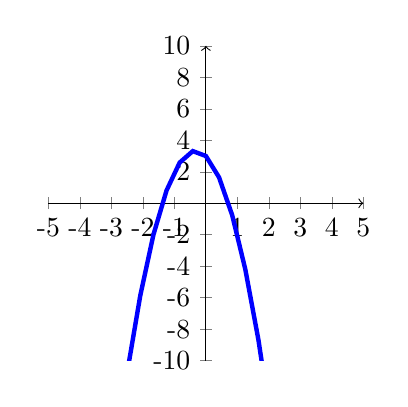
\begin{tikzpicture}
\begin{axis}[
    xmin=-5, xmax=5,
    ymin=-10, ymax=10,
    axis lines=center,
    axis on top=false,
    domain=0:1,
    x=0.4cm,
    y=0.2cm,
    xtick={-5,-4,...,5},
    xticklabels={-5,-4,...,5},
    ytick={-10,-8,...,10},
    yticklabels={-10,-8,...,10},
    axis lines=middle,
    axis line style={->},
    %x label style={at={(axis description cs:0.5,-0.1)},anchor=north},
    %y label style={at={(axis description cs:-0.1,.5)},rotate=90,anchor=south},
    %xlabel={$x$},
    %ylabel={$x^2$},
    %grid=major
    ]
	\addplot [blue,ultra thick,domain=-5:5] {-3*x^2 - 2*x + 3};
\end{axis}
\end{tikzpicture}\\
$a=-0.5$, $b=1$, $c=-2$ \hspace*{0.5in} & \hspace*{0.5in} $a=-3$, $b=-2$, $c=3$\\
$-0.5x^2 + x - 2$ \hspace*{0.5in} & \hspace*{0.5in} $-3x^2 - 2x + 3$\\
\end{tabular}
\end{center}

There's no need to study this chart in much detail, but we can quickly gather a few observations by comparing the values of $a$, $b$, and $c$:
\begin{itemize}
\item When $a$ changes, the shape of the curve changes.  More specifically,
\begin{itemize}
\item When $a$ is positive, the curve opens upward; when $a$ is negative, the curve opens downward.
\item Larger values of $a$ (in magnitude) make the curve narrower (taller); smaller values of $a$ make the curve wider (shorter).
\end{itemize}
\item When $b$ and $c$ change, the location of the curve changes.
\begin{itemize}
\item Increasing $c$ moves the curve upward; decreasing $c$ moves it downward.
\item The effect of $b$ is harder to see, but it, in combination with $a$ and $c$, moves the curve both vertically and horizontally.
\end{itemize}
\end{itemize}

The most important takeaway from this comparison is probably the effect of $a$.  When we start fitting parabolas to data, the value of $a$, the number multiplied by $x^2$ or $t^2$, will tell us the direction of the curve, as well as something about how steep the curve is.

With this background, we're ready to state the formula that we can use to describe data with a quadratic model.

\begin{formula}{Quadratic Growth Models}
The following formula can be used to make predictions when data follows an approximately parabolic trend:
\[P_t = at^2 + bt + c\]
The values of $a$, $b$, and $c$ control the shape and location of the curve.
\end{formula}

Notice that we use $t$ in the formula, to match the formulas in the other sections in this chapter, but we'll use $x$ interchangeably with $t$ in the problems we do, since we'll use calculators and other technology to solve these problems, and those tools generally use $x$ as the variable.
\vfill
\pagebreak

\subsection{Using the Calculator}

\begin{example}[https://www.youtube.com/watch?v=N97Qj97Siec&list=PLfmpjsIzhztutjEb8Pg5OBOlI1p80yVoy&index=5]{Plotting Points on a Calculator}
\marginnote{
\includegraphics[width=1.2in]{OldPeople}}
According to the U.S. Census Bureau, the number of Americans over the age of 100 is increasing.  The Census Bureau reported the following data, where the number of people is measured in the thousands:
\begin{center}
\begin{tabular}{c c}
\textbf{Year} & \textbf{Number}\\
& \textbf{(thousands)}\\
\hline
& \\
1994 & 50\\
1996 & 56\\
1998 & 65\\
2000 & 75\\
2002 & 94\\
2004 & 110
\end{tabular}
\end{center}

Graph this data using a graphing calculator.

\sol
To begin, we need to enter the data, using the same steps outlined in the previous section.  Press the \calcbutton{STAT} button to enter the statistics menu, press \calcbutton{ENTER} to enter the data entry menu, and add the values in the table above to the table in the calculator.  Use the same order in the columns.

\paragraph{Note: order of the columns} This is discussed more in the Statistics chapter, but the first column generally refers to the variable that we use to predict the other.  In this case, we can predict the number of Americans over the age of 100 by picking a given year.  We would be less likely to predict what year we're describing based on the number of Americans over the age of 100.\\

We'll use 1994 as the beginning of our experiment, so that will correspond to year 0.  Once you enter the data, you should see the following.
\begin{center}
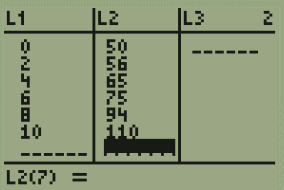
\includegraphics[width=2in]{AgeExample1}
\end{center}

To graph this data, we need to use the \texttt{STAT PLOT} option, which is the \texttt{2ND} option on the \calcbutton{Y=} button, so to access it, press \calcbutton{2ND} followed by \calcbutton{Y=}\ .  This opens the following menu.
\begin{center}
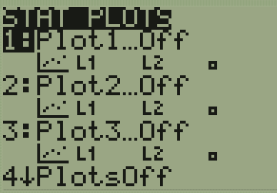
\includegraphics[width=2in]{AgeExample2}
\end{center}

Pressing \calcbutton{ENTER} opens the menu for the first plot.  In order to display a statistics plot, you must turn it on (and turn it off later if you'd like to only graph a function).
\pagebreak

There are various types of statistics plots that the calculator can draw, but the first option (the one selected as shown) is a scatterplot, which is what we want.  Leave the rest of the options as they are (note the order of the data columns).

\begin{center}
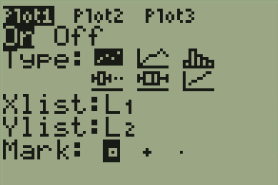
\includegraphics[width=2in]{AgeExample3}
\end{center}

We must zoom the window properly to ensure that we can see the data as it is graphed; the values shown below work well.

\begin{center}
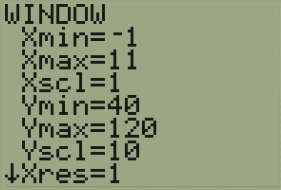
\includegraphics[width=2in]{AgeExample4}
\end{center}

Now, if you press \calcbutton{GRAPH} you should see the following:

\begin{center}
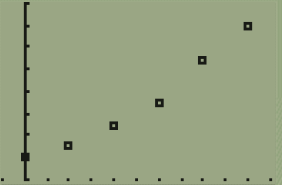
\includegraphics[width=2in]{AgeExample5}
\end{center}

Notice that the shape is similar to the parabolas we have seen drawn, or at least a portion of one.
\end{example}

\begin{try}
Use a graphing calculator to plot the data below, and see if it follows an approximately quadratic trend.
\begin{center}
\begin{tabular}{c c}
$x$ & $y$\\
\hline
0.9 & 2.5\\
1.3 & 4.1\\
1.6 & 5.1\\
2.1 & 7.5\\
2.5 & 9.8\\
3.2 & 14.3\\
3.6 & 18.1\\
4.2 & 23.0
\end{tabular}
\end{center}
\end{try}

The next question, of course, is how to fit a quadratic model to data like this.  Specifically, this means finding values for $a$, $b$, and $c$ that will make the resulting curve match the data as closely as possible.

Unlike with linear models, we won't do this manually, since the algebra necessary is more complicated than we'd like to tackle here.  Thus, we will simply take advantage of the \textbf{quadratic regression} option on the calculator, which is labeled \texttt{QuadReg}.

This can be found in the same menu as the linear regression function, and the process is very similar as well.
\pagebreak

\begin{example}[https://www.youtube.com/watch?v=mFMqHx1lmEE&list=PLfmpjsIzhztutjEb8Pg5OBOlI1p80yVoy&index=6]{Fitting a Quadratic Model on a Calculator}
Using the same census data as in the previous example, find a quadratic model that can be used to predict how many Americans will be over the age of 100 in a given year.

\sol
First, we must have the data entered, so if you don't have the data still in your calculator, follow the first step of the previous example to enter it.\\

Next, press the \calcbutton{STAT} button and use the right arrow button to move to the \texttt{CALC} menu.  There you should find an option labeled \texttt{5: QuadReg} that will perform quadratic regression.

\begin{center}
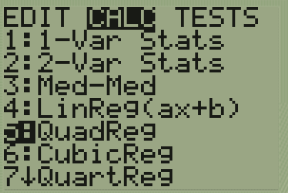
\includegraphics[width=1.7in]{AgeExample6}
\end{center}

If you entered the year in the first column and the number of people in the second column, you won't have to change anything on the next menu.  Simply scroll down to \texttt{Calculate}, and press \calcbutton{ENTER}

\begin{center}
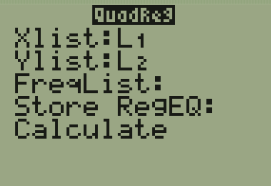
\includegraphics[width=1.7in]{AgeExample7}
\end{center}

The results are shown below.

\begin{center}
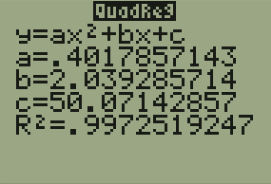
\includegraphics[width=1.7in]{AgeExample8}
\end{center}

Based on the values of $a$, $b$, and $c$ given, we get the following model:
\[\boxed{P_t = 0.40t^2 + 2.04t + 50.07}\]
\end{example}

\begin{try}[http://hartleymath.com/versatilemath/tryit/\#/growth-models--quadratic-regression]
Use a graphing calculator to find a quadratic model for the data given below.
\begin{center}
\begin{tabular}{c c}
$x$ & $y$\\
\hline
0.9 & 2.5\\
1.3 & 4.1\\
1.6 & 5.1\\
2.1 & 7.5\\
2.5 & 9.8\\
3.2 & 14.3\\
3.6 & 18.1\\
4.2 & 23.0
\end{tabular}
\end{center}
\end{try}
\pagebreak

\begin{example}[https://www.youtube.com/watch?v=FemfjoeQ0hk&list=PLfmpjsIzhztutjEb8Pg5OBOlI1p80yVoy&index=7]{Making Predictions with a Quadratic Model}
A study designed to track the gas mileage of a car based on its speed found the following results.
\begin{center}
\begin{tabular}{c c}
\textbf{Speed (mph)} & \textbf{Mileage (mpg)}\\
\hline
& \\
15 & 22.3\\
20 & 25.5\\
25 & 27.5\\
30 & 29.0\\
35 & 28.8\\
40 & 30.0\\
45 & 29.9\\
50 & 30.2\\
55 & 30.4\\
60 & 28.8\\
65 & 27.4\\
70 & 25.3\\
75 & 23.3
\end{tabular}
\end{center}

\begin{enumerate}[(a)]
\item Use a graphing calculator to plot the data.
\item Find a quadratic model that best fits the data.
\item Based on this model, what gas mileage should be expected at 62 miles per hour?  At 90 miles per hour?  Which of these predictions is likely to be more reliable?
\item Based on the model, what speeds are likely to produce a mileage of 28 miles per gallon?
\end{enumerate}

\sol
\begin{enumerate}[(a)]
\item Follow the steps outlined in the first example, and you should see the graph shown below.
\begin{center}
\begin{tabular}{c c c}
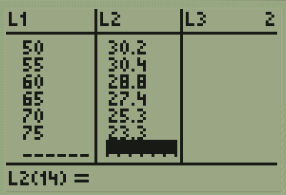
\includegraphics[width=1.3in]{MileageExample1}
& 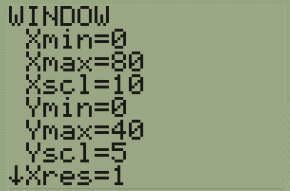
\includegraphics[width=1.3in]{MileageExample2}
& 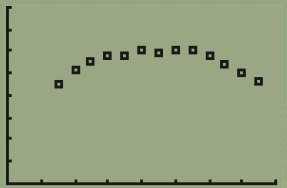
\includegraphics[width=1.3in]{MileageExample3}
\end{tabular}
\end{center}

\item Under the \texttt{STAT} $\longrightarrow$ \texttt{CALC} menu, use the \texttt{QuadReg} option, leaving all the options unchanged:
\begin{center}
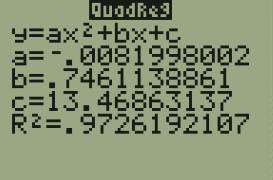
\includegraphics[width=2in]{MileageExample4}
\end{center}
The model found by the calculator is \[\boxed{P_t = -0.008t^2 + 0.746t + 13.469}\]
\pagebreak

\item To make predictions for the mileage ($P_t$) based on speed ($t$), simply substitute those values into the model:
\begin{itemize}
\item At 62 mph: $P_t = -0.008(62)^2 + 0.746(62) + 13.469 = \boxed{28.97 \textrm{ mpg}}$
\item At 90 mph: $P_t = -0.008(90)^2 + 0.746(90) + 13.469 = \boxed{15.81 \textrm{ mpg}}$
\end{itemize}

Which of these seems more likely to be reliable?  The main difference between the two is that 62 mph falls within the range of speeds for which we have data, while 90 mph is faster than anything that was tested.  Thus, we can call the first prediction (at 62 mph) an \textbf{interpolation} and the second an \textbf{extrapolation}.  In general, interpolations are more reliable, because there may be effects we haven't observed outside the range we tested for.

\item To find the speeds that match a mileage of 28 mpg, we need to solve
\[28 = -0.008t^2 + 0.746t + 13.469\]
Rather than doing this algebraically, we can use the same tool we used for this kind of problem in the last section: graph both sides of the equation and use the intersect tool on the calculator.  Notice that there are two intersections this time, so we need to move the cursor close to the second intersection when we want to find that point.
\begin{center}
\begin{tabular}{c c c}
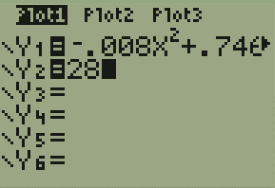
\includegraphics[width=1.3in]{MileageExample5}
& 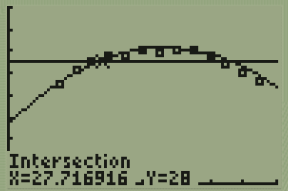
\includegraphics[width=1.3in]{MileageExample7}
& 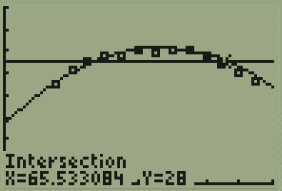
\includegraphics[width=1.3in]{MileageExample8}
\end{tabular}
\end{center}

The two speeds that we would expect to produce a gas mileage of 28 mpg are $\boxed{27.7 \textrm{ mph}}$ and $\boxed{65.5 \textrm{ mph}}$
\end{enumerate}
\end{example}

\begin{try}[http://hartleymath.com/versatilemath/tryit/\#/growth-models--quadratic-regression]
Use the data and model from the previous TRY IT example.

\begin{enumerate}[(a)]
\item Predict the values of $y$ if $x=3$ and if $x=9$.  Which prediction is more likely to be reliable?
\item Find the value(s) of $x$ that match $y=10$ according to that model.
\end{enumerate}
\end{try}

\subsection{Using Excel}
The process for using Excel with quadratic models is almost identical to the one shown in the last section for linear models.  To illustrate, we'll use the dataset from the last example, with the relationship between speed and gas mileage.

First, record the data and insert a scatterplot, as before.
\begin{center}
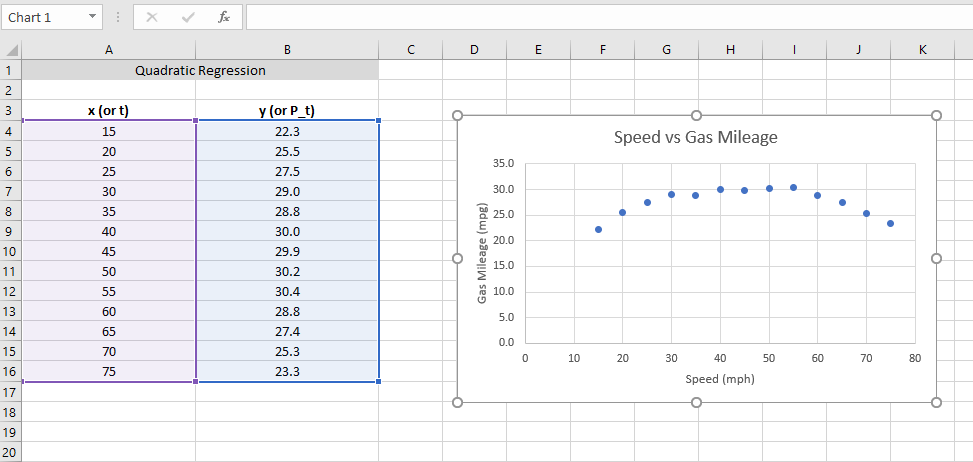
\includegraphics[width=0.8\textwidth]{MileageExcelExample1}
\end{center}

Next, click the plus sign in the upper right corner of the chart, and at the bottom of the menu, click the arrow next to the ``Trendline'' option and select ``More Options...''
\begin{center}
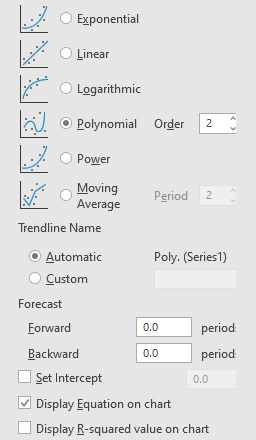
\includegraphics[width=1.5in]{MileageExcelExample2}
\end{center}

This time, instead of selecting the linear option, select ``Polynomial'' with order 2 (that's the squared part of a quadratic model).  As always, select the option to display the equation on the chart.
\begin{center}
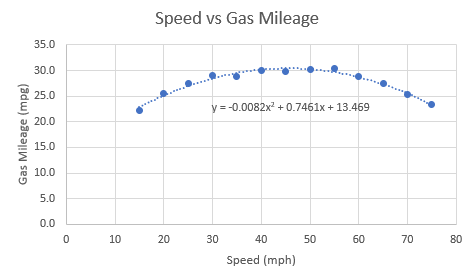
\includegraphics[width=0.8\textwidth]{MileageExcelExample3}
\end{center}